%\documentclass{Latex_Euclid_style}

%\usepackage{amsmath}
%\usepackage{amsfonts}
%\usepackage{amssymb}
%\usepackage{graphicx}
%\usepackage{epsfig}
%\usepackage[hang,small,bf]{caption}
%\usepackage{rotating}


% --------------

%\begin{document}

\section{Splinter Group 1: numerical codes}

\subsubsection*{Coordinators}
\begin{itemize}
 \item Valeria Pettorino, Matteo Martinelli
\end{itemize}
\subsubsection*{Participants}
\begin{itemize}
 \item Matteo Costanzi,  Yabebal Fantaye, Ken Ganga, Martin Kunz, Massimiliano Lattanzi, Julien Lesgourgues, Baojiu Li, Matteo Martinelli, Federico Marulli, Valeria Pettorino, Anna M. Porredon, Marco Raveri, Ziad Sakr, Valentina Salvatelli, Barbara Sartoris, Bj\"orn Malte Schaefer, Luca Amendola, Thejs Brinckmann, Mariana Penna-Lima.
\end{itemize}

\subsubsection*{Aim}
Make a recommendation on existing codes for Atomistic Forecasting approach.\\
Expected output:
\begin{itemize}
 \item A technical note explaining pros and cons of the various potential public codes for this purpose 
 \item How do they meet our requirements:
 \begin{itemize}
  \item on the division/requirements setting at fine-grained level 
  \item on individual probe work and on combinations
 \end{itemize}
 \item Make a consensus of codes, and make a short presentation showing initial pros and cons.
\end{itemize}

\newpage
\subsection{Boltzmann codes}
This section includes an overview of publicly available Boltzmann codes. For each code we present a schema in the same format, including pros and cons.



\newpage
\subsubsection{CAMB}
%\href{http://camb.info/}{CAMB}
(\url{http://camb.info/})\\

{\it \bf Language:} fortran90\\

{\it \bf Includes:}
\begin{itemize}
 \item standard neutrinos, sterile neutrinos
 \item CDM
 \item DE: $w_0\ w_a$
\end{itemize}

{\it \bf Pros: }
\begin{itemize}
%publicly available
 \item updated very often
 \item tested by a large community
 \item there are several implementations for MG models (though not as well tested)
 \item python wrapper for CAMB to join to any MCMC
 \item documentation available and often updated: quick feedback by Anony Lewis and large community, via cosmocoffee
\end{itemize}

{\it \bf Cons:}
\begin{itemize}
 \item structure of the code requires to modify different parts of the code for different models
 \item no general distribution function for neutrinos
 \item only synchronous gauge
 \item maintainer (Antony Lewis) not currently in Euclid
\end{itemize}

\newpage
\subsubsection{EFTCAMB}
(\url{http://wwwhome.lorentz.leidenuniv.nl/~hu/codes/}\\
\url{https://github.com/EFTCAMB/EFTCAMB})\\

{\it \bf Language:} fortran90\\

{\it \bf Includes:}\\
\begin{itemize}
\item parametrized pure EFT approach to Horndeski (including the $\alpha$ parameterization), GLPV (?), 
      Horava-Lifshitz 
\item exact (mapping) implementation of: designer f(R), Hu-Sawicki f(R), low-energy Horava
\item several backgrounds and massive neutrinos
\end{itemize}


{\it \bf Pros:}
\begin{itemize}
 \item based on CAMB
 \item very general parametrization of the effective field theory (EFT) parametrisation of MG and DE models
 \item tested against HiCLASS/MGCAMB/private codes for some models
 \item several parameterisations of the background expansion and also of the perturbations (including Horndeski and beyond (e.g. GLPV))
 \item perturbation evolution computed self-consistently for EFT class of models
 \item Very clearly written, structured, documented. 
 \item It has a MCMC wrapper.
 \item maintainers are active Euclid members
\end{itemize}

{\it \bf Cons: }
\begin{itemize}
 \item need further testing
 \item needs further development and understanding of the stability conditions
 \item MG starts from z = 100 (not tested earlier)
\end{itemize}

\newpage
\subsubsection{MGCAMB}(\url{http://aliojjati.github.io/MGCAMB/})\\

{\it \bf Language:} fortran90\\

{\it \bf Includes: }
\begin{itemize}
 \item Parametrization of linear scalar perturbations in DE/MG based on two functions of time and scale ($\mu, \gamma$ (or Q,R).
\item LCDM and \textcolor{red}{general w(z) (To be checked)}
\item massive neutrino
\item Linder gamma parametrisation of the growth rate
\item can treat the following specific models in the quasi-static approximation: BZ parametrization of f(R), (beta, m) parametrisation of Generalized Brans-Dicke, Hu-Sawicki f(R), Generalized Brans-Dicke (including symmetron and dilaton models)

\end{itemize}

{\it \bf Pros: }
\begin{itemize}
 \item it works with some well tested parametrization; easy to compare with previous results 
 \item can test  very general deviations from LCDM visible in the scalar metric perturbations
 \item  It has MCMC wrapper
\end{itemize}

{\it \bf Cons: }
\begin{itemize}
 \item When used as a ‘EFT replacement’:
 \begin{itemize}
  \item does not evolve all perturbation equations 
  \item assumes quasi static limit
 \end{itemize}
 \item General deviations in scalar metric perturbations require careful parameterisation, some further developments (eg. Gaussian process) may be required
 \item Does not include similar deviations in vector and tensor perturbations
 \item Works with $\Lambda$CDM background
\end{itemize}
Warning: the code was recently updated (late february). These comments do not refer to the latest version.\\

\newpage
\subsubsection{CLASS}(\url{http://class-code.net/})\\

{\it \bf  Language:} C

{\it \bf Includes:}
\begin{itemize}
 \item various forms of neutrinos and dark matter
 \item DE with a given equation of state, quintessence with scalar potentials.
 \item DE extension is HiClass but not public (Bellini, Miguel Zuma)
 \item newtonian and synchronous gauge
\end{itemize}

{\it \bf Pros: }
\begin{itemize}
 \item structure of code
 \item python wrapper
 \item two gauges (newtonian and synchronous: except the initial conditions which are only written in the synchronous gauge and gauge-transformed). 
 \item maintainer (Julien Lesgourgues) is active Euclid member
\end{itemize}

{\it \bf Cons: }
\begin{itemize}
 \item community that uses/tested CLASS is smaller than CAMB
\end{itemize}


\newpage

\subsection{Parameter estimation codes}
This subsection includes an overview of publicly available codes to calculate the likelihood.

\subsubsection{Wish list definition}

The basic requirement for codes which obtain cosmological predictions from Boltzmann codes and perform parameter estimation is ``modularity''.\\
A modular code is easy to modify in case some changes and updates need to be included, e.g. additional likelihoods, extra parameters, correction to observables (systematics).\\
Furthermore, separate modules for different physical quantities are needed for the atomistic approach as they allow to easily retrieve and compute the intermediate quantities of the theory
flows (see e.g. Fig. \ref{WLtomo}) and to compare them between different codes.\\
However too much modularity may affect code performances.\\

The wish list of modules is:
\begin{enumerate}
 \item module calling the Boltzmann/transfer function codes for primary science
 \item module calling the sampler
 \item module for each likelihood for each probe
 \item module for background quantities
 \item module for perturbation quantities
 \item module for non-linear corrections (ex. halofit)
 \item module that gets the standard output from Boltzmann codes and produces list of suitable output
 \item postprocessing of the samples
 \item plotting modules 
 \item module for cross correlation of probes
\end{enumerate}

In the following, the publicly available codes are listed, together with the requirements which are satisfied by each of them. The missed requirements are also listed and the complexity 
of implementation is indicated as easy (E), medium (M) and difficult (D).

\newpage
\subsubsection{COSMOMC}
(\url{http://cosmologist.info/cosmomc/})\\

{\it \bf Language:} fortran90\\

{\it \bf Includes:}\\
\begin{itemize}
\item SN: JLA, Union
\item CMB+CMB Lensing: Planck, WMAP, BICEP2+Keck
\item LSS: WiggleZ, SDSS LRG, CFHTLenS
\item BAO+RSD: several (noticeably BOSS)
\item HST H0 measurements
\item SZ CLUSTER: Planck
\end{itemize}

{\it \bf Pros:}
\begin{itemize}
 \item updated constantly
 \item very well tested, very efficient for standard cosmology
 \item used by a large community
 \item easy to add parameters
 \item easy to add an additional likelihood by adding a separate module
 \item nice python graphical interactive interface for first tests
 \item well documented
 \item there are many options and more control to analyse the samples. 
 \item Updated to all currently available data (WL, GC, clusters, CMB).
 \item Likelihood Sampler works really well
\end{itemize}

{\it \bf Cons: }
\begin{itemize}
 \item if you increase the number of parameters, the sampler gets slower. Other samplers are publicly available and already interfaced with COSMOMC. However they are not included in the 
 standard version (interface needs to be modified when COSMOMC is updated)
 \item maintainer (Antony Lewis) not currently in Euclid
\end{itemize}

{\it \bf Wish-list requirements: }
\begin{itemize}
 \item included: 1, 2 (add samplers), 3, 6, 8, 9
 \item missing: 4 (E CAMB has background functions collected in module ModelParams in modules.f90 which can be called by COSMOMC), 5 (D), 6 (alternatives to halofit), 7 (E/M)
\end{itemize}

\newpage
\subsubsection{MONTEPYTHON}(\url{https://github.com/baudren/montepython_public} or \url{http://baudren.github.io/montepython.html})\\

{\it \bf Language:} python\\

{\it \bf Includes:}
\begin{itemize}
 \item Euclid mock likelihood (weak lensing + galaxies) is publicly available
 \item CMB, SNIa, BAO, WiggleZ (CHFTLens and SDSS to be released); 
\end{itemize}

{\it \bf Pros: }
\begin{itemize}
 \item modular environment
 \item can switch among different samplers
 \item it has a graphical interface
 \item can easily be interfaced with different Boltzmann codes
 \item can use MPI
 \item extra parameters need to be included only in the input file
 \item easy to add a new likelihood.
\end{itemize}

{\it \bf Cons:} 
\begin{itemize}
 \item community that uses/tested MP is smaller than COSMOMC
 \item less frequently updated 
\end{itemize}

{\it \bf Wish-list requirements: }
\begin{itemize}
 \item included: 1 (for generic Boltzmann code; currently points at Class wrapper; Camb wrapper in preparation), 2 (MH, Multinest, CosmoHammer, importance sampling, reprocessing chains, fisher matrices), 3, 4, 5, 6 (Halofit), 7, 8, 9 (can choose between MontePython or Getdist to produce plots or reprocess: chains are in the same format as cosmomc and can use 8,9 from COSMOMC) 
 \item missing: 6 (alternatives to Halofit E/M) 
\end{itemize}

\newpage
\subsubsection{COSMOSIS}
(\url{https://bitbucket.org/joezuntz/cosmosis/wiki/Home})\\

{\it \bf Language:} Written in C++ and python. Modules can be written in C, C++, Fortran, or Python.\\

{\it \bf Includes: }
\begin{itemize}
\item the models discussed here: \url{https://bitbucket.org/joezuntz/cosmosis/wiki/default_modules}
 \item Different samplers: including emcee (see schema discussed in this document), fisher matrices sampler and Multinest (that computes the Bayesian evidence and the posterior pdf's.) http://arxiv.org/pdf/1409.3409v1.pdf
 \item Likelihoods are listed here: \url{https://bitbucket.org/joezuntz/cosmosis/wiki/default_modules} in the likelihood section.
 \item CAMB, CLASS
\end{itemize}

{\it \bf Pros:} 
\begin{itemize}
 \item can be wrapped to CAMB and CLASS
 \item it is modular (can introduce other samplers or Boltzmann codes or likelihoods) 
 \item can add modules in different languages
 \item new parameters are defined only in the input parameter file
 \item They will include SDSS. Easy to implement a new module for a new likelihood.
 \item Used by DES.
 \item Issues are usually rapidly answered in the issues tab of the bitbucket repository.
 \item Postprocess tool that automatically makes python plots of the sampler outputs (some demos: \url{https://bitbucket.org/joezuntz/cosmosis/wiki/Home})
\end{itemize}

{\it \bf Cons:} 
\begin{itemize}
 \item not very well tested
 \item small community uses it
 \item Not clear how often it is updated (Responsible is: Joe Zuntz et al, not in Euclid).
 \item Quality of demos visualisation seems lower than available for getdist python plotting.
\end{itemize}

{\it \bf Wish-list requirements: }
\begin{itemize}
 \item included: 1 (generic Boltzmann code: CAMB, CLASS), 2 (MH, MultiNest, EMCEE), 3 (...add…), 4 (?), 6 (Halofit, Halofit + T correction), 7
 \item Datablock the object passed down the pipeline. For a given set of parameters all module inputs are read from the datablock and all module outputs are written to it 
 \item missing: 4 (E but not implemented?), 5 (?), 6 (alternatives to Halofit; E/M), 8 (format of chains? can one use getdist? how advanced as compared to getdist?), 9 
 (how advanced with respect to COSMOMC ones?) 
\end{itemize}

\newpage
\subsubsection{NumCosmo}

(\url{http://www.nongnu.org/numcosmo/})\\
(\url{https://github.com/NumCosmo/NumCosmo}) \\

{\it \bf Language:} C (main), Python, Perl, Java, Java Script, Vala, Lua, Ruby (for a complete list see \url{https://wiki.gnome.org/Projects/GObjectIntrospection/Users})
\\

{\it \bf Includes:}
\begin{itemize}
 \item some BAO, some H(z) , SNe Ia JLA,  Planck, some cluster data
\item resample codes (from a probability density function and  bootstrap)
\item sampler codes
\end{itemize}

{\it \bf Pros:} 
\begin{itemize}
 \item modular environment
 \item	can switch among different samplers
 \item MCMC object is modular and one can implement just a new transition kernel
\item 	can easily be interfaced with different Boltzmann codes
\item 	the code is parallelized through multithread and easily extended to MPI
\item 	all parameter information is defined in the NcmModel. It is inherited by NcmMSet, NcmFit, NcmFitMCMC etc, avoiding repetition
\item 	easy to add a new likelihood
\item 	it call be called from any bind language or from a general purpose executable (in C) called darkenergy
\item 	frequently updated
\item 	portable to Linux, Mac OS and Window
\item 	it uses autotools as its building system allowing NumCosmo to be easily compiled in several architectures
\item 	a list of pre-compiled packages can be found at https://build.opensuse.org/package/show/home:vitenti/numcosmo
\item 	the QA is assured by a set of tests using ''Unit testing''

 \end{itemize}

{\it \bf Cons:} 
\begin{itemize}
 \item 	community that uses/tested NumCosmo is much smaller than COSMOMC
 \item 	external dependencies (NLopt, Sundials, cfitsio, etc)
 \item 	users can call NumCosmo from any bind language, but the developers have to learn GObject and GObject Introspection. We plan to provide a cookbook to make it easier.
 \item 	no graphical interface
 \end{itemize}

{\it \bf Wish-list requirements: }
\begin{itemize}
 \item included: 1 (CLASS wrapper, generic Boltzmann code in progress); 2 (statistical tools available: best-fit finders, Fisher Matrix,  Monte Carlo (resample from a probability density function and bootstrap), Profile Likelihood, Markov Chain Monte Carlo (Metropolis-Hastings, Ensemble sampler MCMC), Approximate Bayesian Computation); 3; 4; 5; 6 (halofit, halo model); 7; 8; 9.
\end{itemize}

\newpage
\subsubsection{ITAbox} 



{\it \bf Language:} python\\

{\it \bf Includes:}
\begin{itemize}
\item uses emcee as sampler (\url{http://dan.iel.fm/emcee/current/}); plotting tools
\end{itemize}

{\it \bf Pros:} 
\begin{itemize}
 \item affine invariant sampling for fast sampling of degenerate likelihoods
 \item parallel tempered sampler for multimodal likelihoods
 \item standard Metropolis-Hastings sampler
 \item many plotting tools included
 \item can use MPI
 \item interfaces reasonbly easy to write
 \item interface to lensing code exists (in C)
 \item interface to supernova code exists (in C or python)
 \end{itemize}

{\it \bf Cons:} 
\begin{itemize}
 \item not specifically interfaced to a Boltzmann code
\end{itemize}

{\it \bf Wish-list requirements: }
\begin{itemize}
\item{included: 2,8,9, 3 (lensing, supernovae and CMB spectra)}
\item{provided: 4, 5}
\item{missing: 1, 3 (iSW-effect, BAO, galaxy density), 6, 7}
\end{itemize}

\newpage

\begin{figure}
    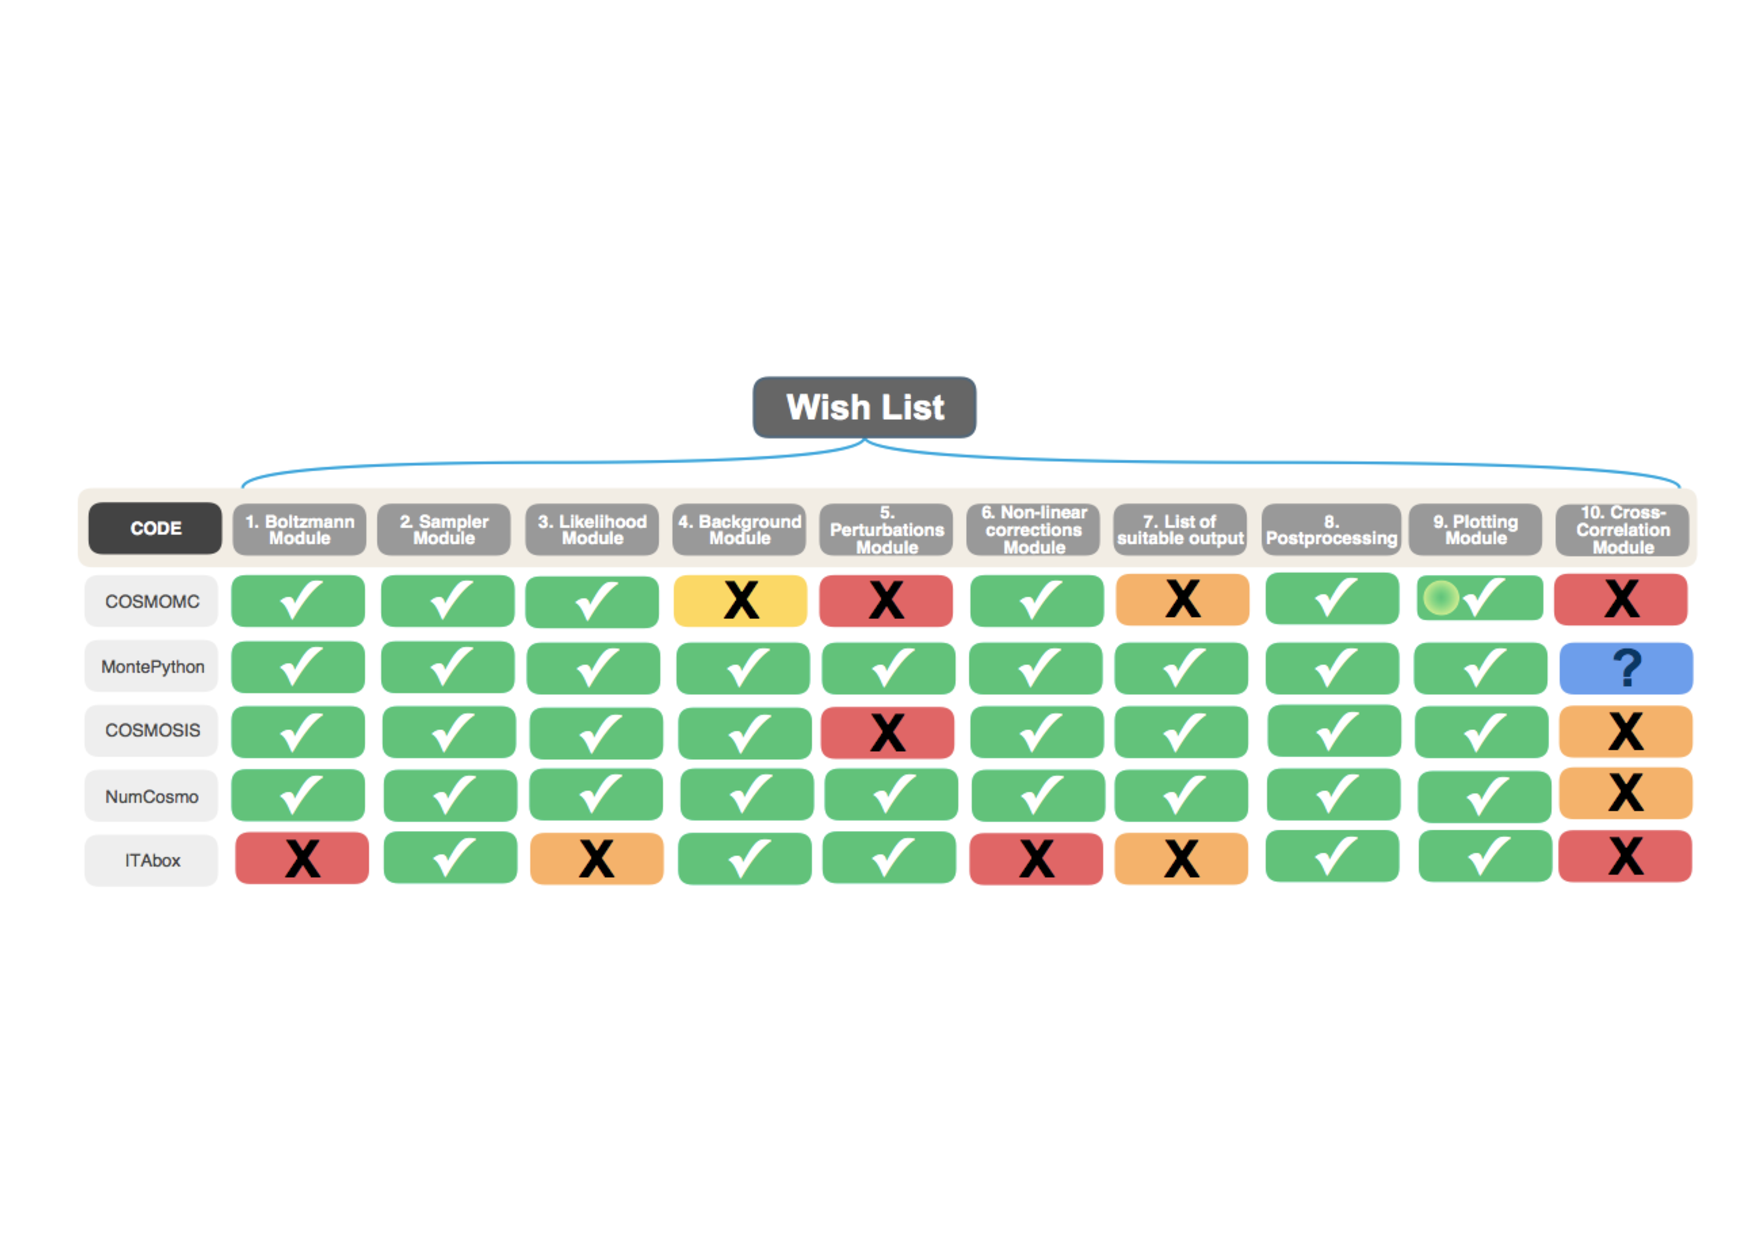
\includegraphics[angle=0,clip=,width=\columnwidth]{IST_codemap.pdf}
 \caption{Likelihood Code Map. Fields correspond to the modules in the wish list. Rows correspond to the numerical codes available and discussed in the text. Easy/Medium?Difficult indicate the estimated level of difficulty to implement the missing modules.}
 \label{ISTcodemap}
\end{figure}
\newpage


\subsection{Recommendation on codes and coding languages to use}

\subsubsection{Coding Language}
The SGS use python and C++ only, and it would be good for us to follow them to have some coherence. Although there are pros and cons.\\
It would be ideal to have a python infrastructure: wrappers in python to other codes written in different open sources free languages (instead of IDL, Mathematica)\\
FR software to convert languages from one to another: help to write a python wrapper, for example SDC is using swig (http://www.swig.org/).
Good experience with SWIG, it serves as a way of passing data between python and other languages (Bjoern: tried out python$\rightarrow$C with openMP-parallelisation)\\
Make sure all libraries used/needed are available. 
SDC already has a list of libraries that are allowed to be used, at \url{http://euclid.roe.ac.uk/projects/codeen-users/wiki/EDEN}.
Python slow for high level performances. 

\subsubsection{Boltzmann code}

No specific choice, but recommendation is that we need at least 2 codes that match for each model (match in the sense explained in the methodology below); 
in addition, our recommendation is to use MGCAMB only for tests (and clearly specify limitations of the code and assumptions in it).


\subsubsection{Parameter estimation and likelihood code map}
A summary of how the likelihood codes compare to the wish list is visualised in Fig.\ref{ISTcodemap}. MontePython is at present the code that includes the highest number of requirements in the wish list. JL \& team within Euclid guarantee fast 
update for wrappers to Boltzmann code version updates and to new data which become available. \\
\textcolor{red}{To be discussed: how the different codes perform on cross correlation of probes.}

\subsubsection{Analysis and visualization}
Getdist and plotting tools provided by cosmomc.

\subsection{Methodology to test a code}

\subsubsection{How to trust a Boltzmann code in Modified Gravity}

For every MG model, there should be at least 2 Boltzmann codes, agreeing. Agreement is defined as follows: 
\begin{itemize}
 \item check them on LCDM, need to agree at less than 0.1\%
 \item check them in a MG scenario in different ranges of parameters: they should match at the same level at which they agree in LCDM on 
all background quantities, all perturbation quantities, all spectra
\end{itemize}

\subsubsection{How to trust a likelihood code}
The code needs to pass a self-consistency check: use a simulation to produce a set of data and check if you can recover the initial cosmological model.\\
Available simulations: \\
galaxy mock catalogue
\begin{enumerate}
 \item from MICE simulations (HOD) in LCDM cosmology  \url{http://internal.euclid-ec.org/?page_id=1551}
 \item from Durham simulations (SAM) in LCDM cosmology 
\end{enumerate}
Needed:
\begin{itemize}
 \item simulations from non-standard cosmological models: e.g. f(R), DE 
 \item simulations with neutrinos
 \item mock catalogue for WL (to be asked to the WL splinter-2)
\end{itemize}


\subsection{Input from other groups}
\subsubsection{SGS}
We need to define the infrastructure of the code pipeline with SGS (\url{http://euclid.roe.ac.uk/projects/sgssu/wiki}), see infrastructure channel on SLACK.
\comment{Contacted Marc Savage}


\subsubsection{Splinter-2}
List of requirements that the ideal CosmoBox code should provide, as for weak lensing.

\paragraph{Specific inputs}
Tomographic redshift distribution, with errors, outlier distributions
Optional: observational effects such as masks
\paragraph{The signal}
Non-linear matter power spectrum down to k ~ 50 h/Mpc (that is where the FoM saturates, Kitching $\&$ Taylor 2011; to model uncertainties in that highly non-linear regime we would then add parameters with certain priors).
Baryonic effects on power spectrum (not clear yet how this should best be implemented) 
Lensing projections: Standard WL power spectrum approximations, optional: second-order corrections
Optional: real-space lensing correlations
\paragraph{Errors}
Gaussian covariance, optional: non-Gaussian covariance
\paragraph{Systematics}
Intrinsic alignment power spectra
Nuisance parameters (e.g. shear biases)

\paragraph{Specific outputs}
Lensing tomographic power spectra, optional: split into different contributions (IA, with/without systematics) for testing


\subsubsection{Splinter-3}

\subsubsection{Splinter-4}

\subsubsection{TWG}
For each model in the parameter definition document (PDD), the TWG provides a table \ref{TWGcodemap} with the following information: Model, code, availability, Reference, Contact person.


\subsection{TWG provided list of models and codes}
\begin{figure}
    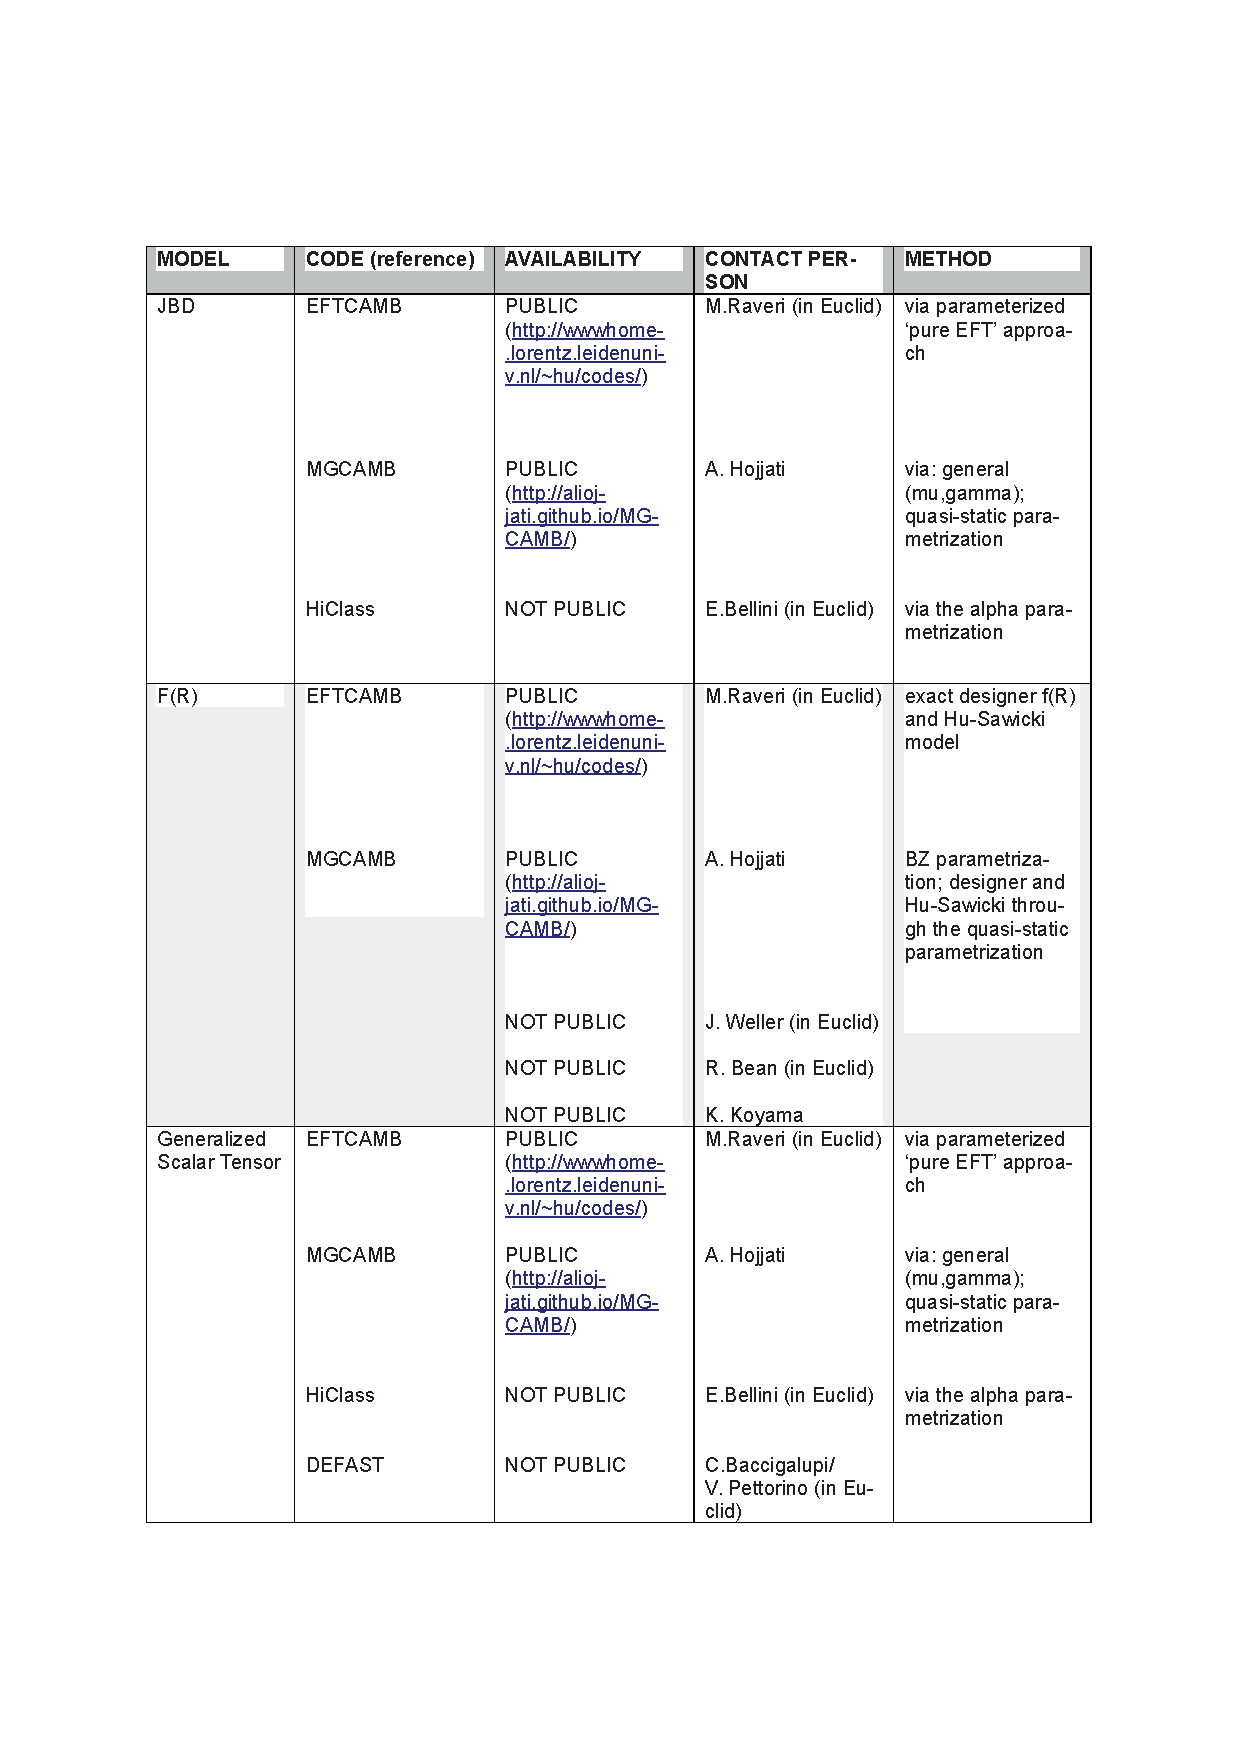
\includegraphics[angle=0,clip=,width=\columnwidth]{Models_and_Codes_1.pdf}
 \caption{TWG models and codes list}
 \label{TWGcodemap}
\end{figure}
\begin{figure}
    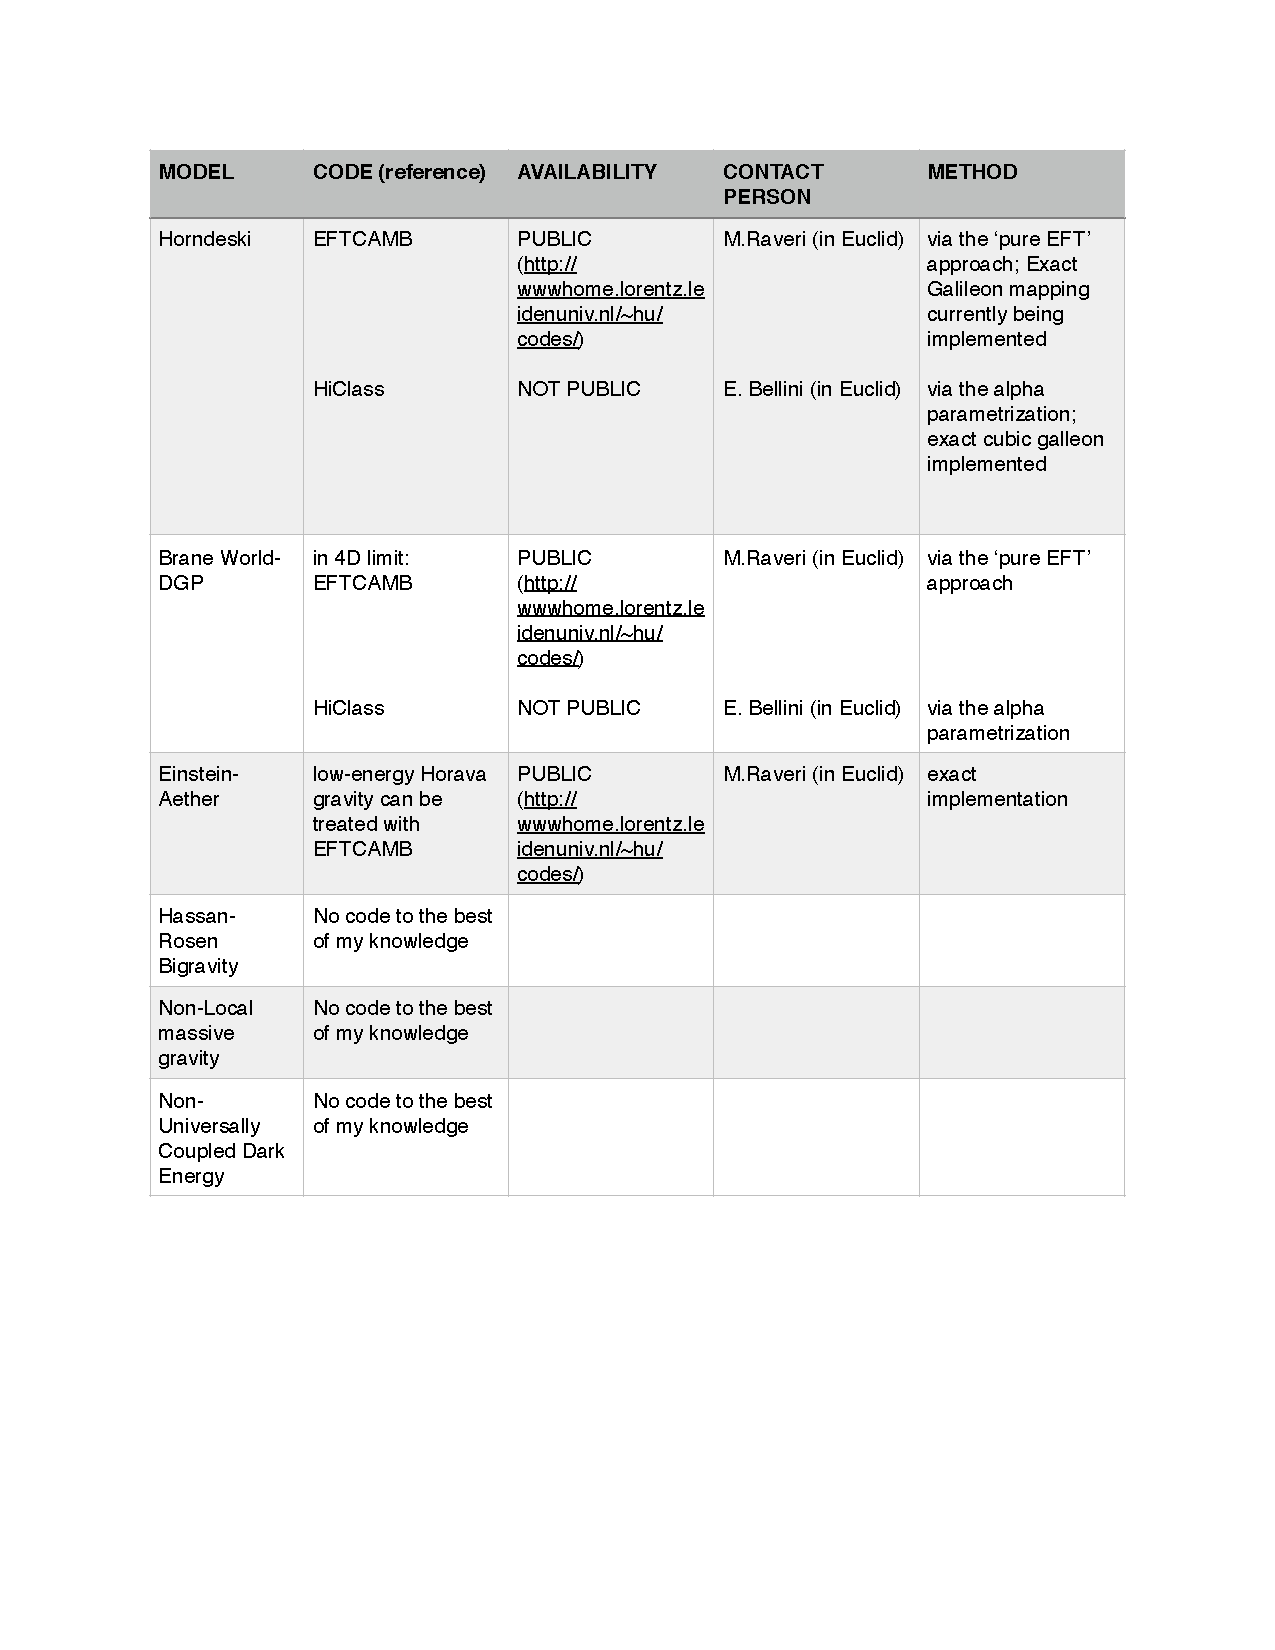
\includegraphics[angle=0,clip=,width=\columnwidth]{Models_and_Codes_2.pdf}
 \caption{TWG models and codes list}
 \label{TWGcodemap}
\end{figure}



\subsubsection{Simulation WG}
The simulation Group provides a table 'model' : 'simulation' : 'reference', where 'simulation' is either 'Not available' or a list of simulations available for the model and 'reference' is the 'reference' contact for that set of simulations.

Model    |     Simulation    |    Reference

LCDM    |     Gadget         | Code: Springel 2005 MNRAS 364, Largest simulation: Millennium XXL, Angulo et al 2012 MNRAS 426

LCDM   |      Ramses     |   Code: Teyssier 2002 A$\&$A 385, Largest Simulation: DEUS FUR, Rasera et al 2014 MNRAS 440

LCDM   |     PKDGRAV    |    Code: Stadel J. PhD Thesis, Largest Simulation:  Euclid Flagship Run (still running)

Code Comparison: Schneider et al. 2015, arXiv:1503.05920



%\end{document}



